\subsubsection{Artificial viscosity smoothing}
\label{sec:artificial-viscosity-smoothing}
\textit{This section was contributed by Ryan Grove}

Standard finite element discretizations of advection-diffusion equations introduce unphysical oscillations around steep gradients. Therefore, stabilization must be added to the discrete formulation to obtain correct solutions. In ASPECT, we use the Entropy Viscosity scheme developed by Guermond et al.~in the paper \cite{guer11}. In this scheme, an artificial viscosity is calculated on every cell and used to try to combat these oscillations that cause unwanted overshoot and undershoot.  More information about how \aspect{} does this is located at \url{https://dealii.org/developer/doxygen/deal.II/step_31.html}.

Instead of just looking at an individual cell's artificial viscosity, improvements in the minimizing of the oscillations can be made by smoothing.  Smoothing is the act of finding the maximum artificial viscosity taken over a cell $T$ and the neighboring cells across the faces of $T$, i.e.,
\begin{equation*}
\bar{v_h}(T) = \max_{K \in N(T)} v_h(K)
\end{equation*}
where $N(T)$ is the set containing $T$ and the neighbors across the faces of $T$.

This feature can be turned on by setting the \hyperref[parameters:Discretization/Stabilization parameters/Use artificial viscosity smoothing]{Use artificial viscosity smoothing} flag inside the \hyperref[parameters:Discretization/Stabilization_20parameters]{Stabilization} subsection inside the \hyperref[parameters:Discretization]{Discretization} subsection in your parameter file.

To show how this can be used in practice, let us consider the simple convection in a quarter of a 2d annulus cookbook in Section \ref{sec:shell-simple-2d}, a radial compositional field was added to help show the advantages of using the artificial viscosity smoothing feature.

By applying the following changes shown below to the parameters of the already existing file \begin{verbatim}cookbooks/shell_simple_2d/shell_simple_2d.prm, \end{verbatim}
\lstinputlisting[language=prmfile]{shell_simple_2d_smoothing.part.prm.out}
it is possible to produce pictures of the simple convection in a quarter of a 2d annulus such as the ones visualized in
Figure~\ref{fig:smoothing}.

\begin{figure}
    \centering
  \subfigure[]{
    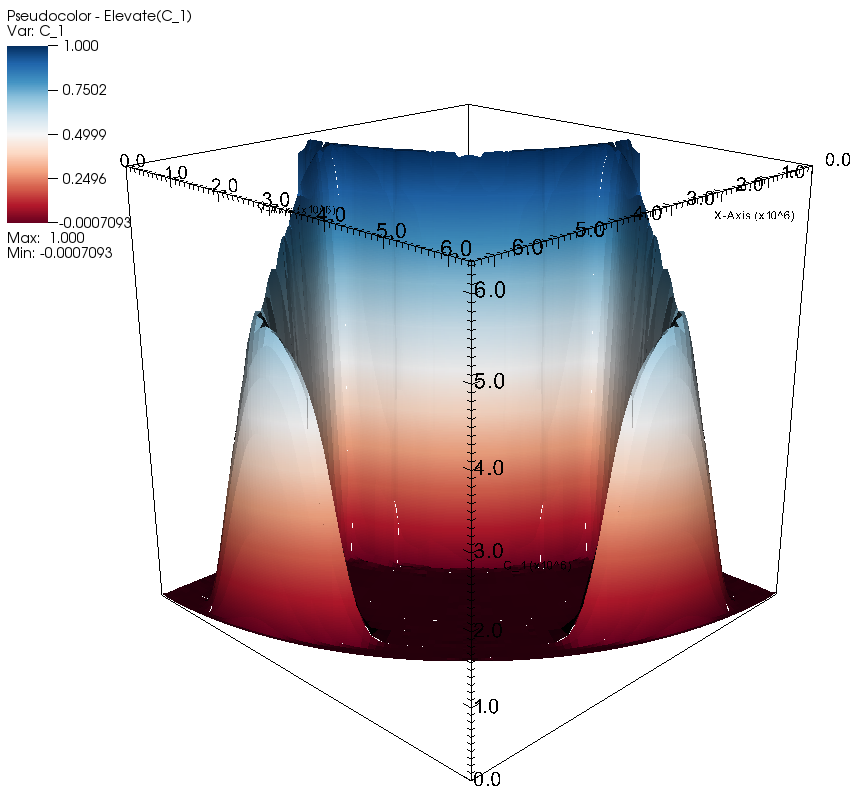
\includegraphics[width=.48\textwidth]{with_smoothing.png}}
  ~
  \subfigure[]{
    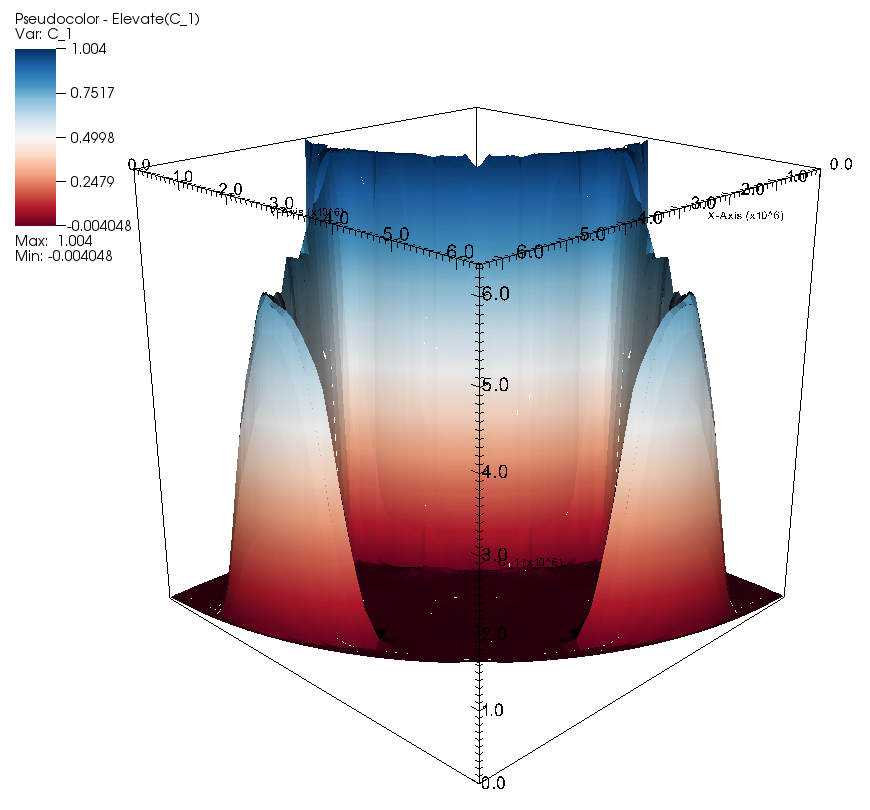
\includegraphics[width=.48\textwidth]{without_smoothing.png}}
    \caption{\it Artificial viscosity smoothing: Example of the output of two similar runs.  The run on the left has the artificial viscosity smoothing turned on and the run on the right does not, as described in Section \ref{sec:artificial-viscosity-smoothing}.}
    \label{fig:smoothing}
\end{figure}


